

\section{Architecture logicielle}

La conception d'une architecture logicielle claire, cohérente et modulaire constitue l’un des piliers fondamentaux de tout projet informatique sérieux. Elle ne se limite pas à organiser du code : elle permet de clarifier les rôles de chaque composant, de faciliter la maintenance du système à long terme, et de rendre possible l’extension ou la réutilisation de tout ou partie du projet dans d'autres contextes.

Dans notre projet, nous avons fait le choix d’une architecture inspirée du paradigme \textbf{MVC} (Modèle – Vue – Contrôleur), une architecture logicielle largement enseignée dans les cours de conception orientée objet et de génie logiciel. Ce modèle vise à séparer les préoccupations :
\begin{itemize}
    \item la \textbf{modélisation des données} (Modèle),
    \item la \textbf{logique de contrôle du système} (Contrôleur),
    \item et l’\textbf{interface graphique avec l’utilisateur} (Vue).
\end{itemize}

Ce découpage offre plusieurs avantages :
\begin{itemize}
    \item il permet de modifier l’interface graphique sans toucher à la logique de traitement,
    \item il permet de faire évoluer la logique du moteur sans impacter les données ni l’affichage,
    \item il facilite le travail collaboratif, chaque membre pouvant se concentrer sur une couche précise.
\end{itemize}

Afin d’illustrer l’organisation générale de notre application avant d’en détailler les parties, nous avons réalisé deux diagrammes UML synthétiques. Ces schémas permettent de visualiser la structure logique du système, les entités clés, ainsi que leurs relations hiérarchiques ou fonctionnelles.

\begin{itemize}
    \item Le premier diagramme présente la vue d’ensemble de l’architecture du projet (niveau système), avec les interactions entre les modules de haut niveau : vue graphique, moteur de simulation, gestion du modèle, etc.
    \item Le second diagramme, plus détaillé, se concentre sur les classes constitutives du modèle : agents, grille, obstacles, états internes, interactions locales, etc.
\end{itemize}

\vspace{1em}

\begin{figure}[H]
    \centering
    \begin{minipage}[b]{0.47\textwidth}
        \centering
        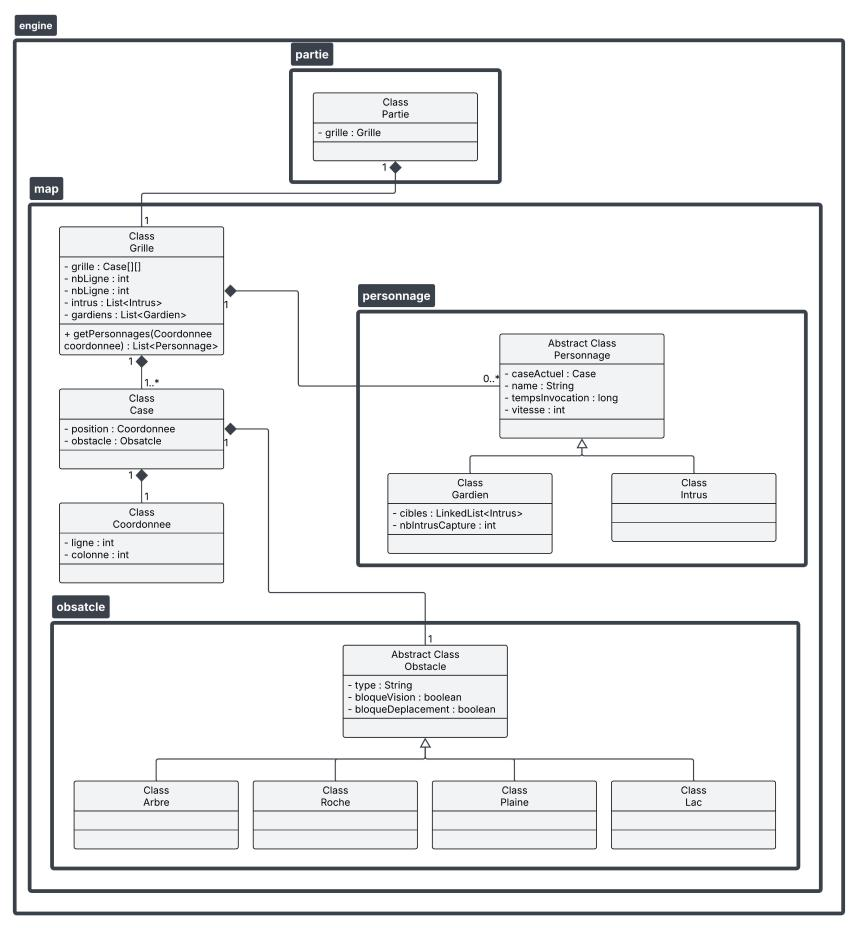
\includegraphics[width=\textwidth]{diag1.jpeg}
        \caption{Diagramme UML global de l’architecture logicielle (MVC)}
        \label{fig:uml-global}
    \end{minipage}
    \hfill
    \begin{minipage}[b]{0.47\textwidth}
        \centering
        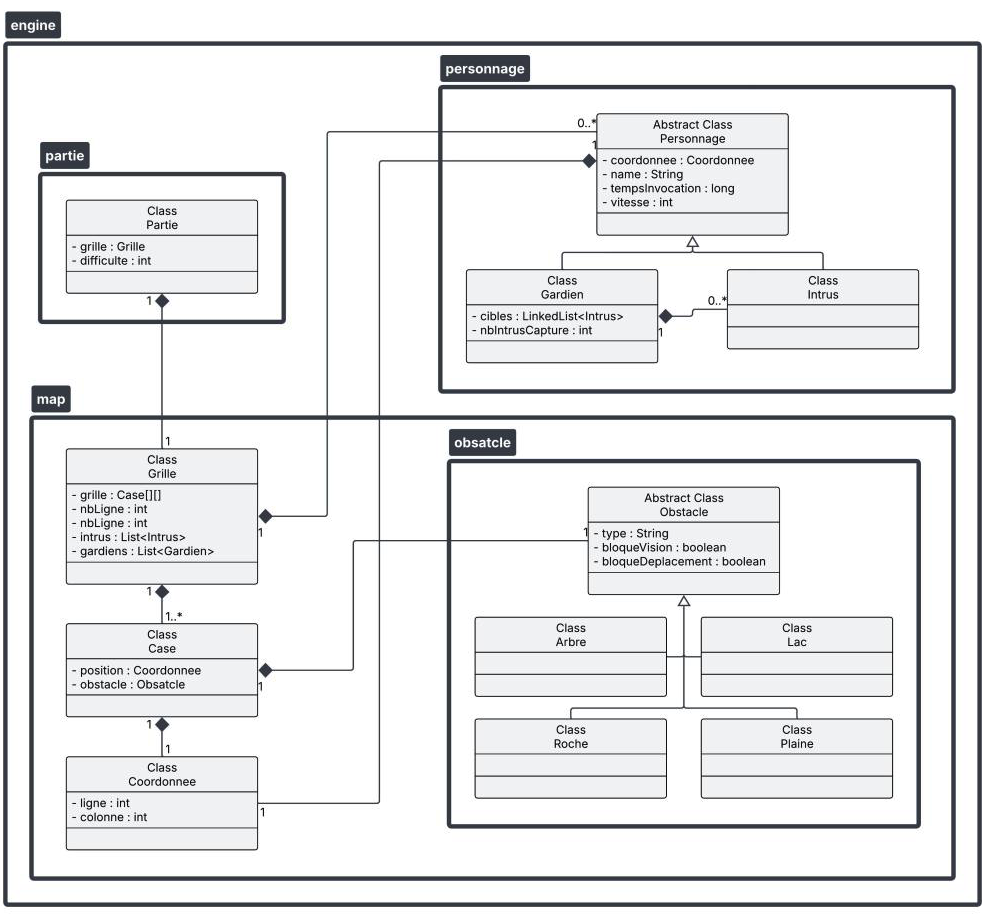
\includegraphics[width=\textwidth]{diag2.png}
        \caption{Diagramme UML du modèle : grille, agents, obstacles}
        \label{fig:uml-modele}
    \end{minipage}
\end{figure}

\vspace{1em}

Ces représentations graphiques ont joué un rôle central dans la conception du projet. Elles nous ont permis :
\begin{itemize}
    \item d’anticiper les interactions entre classes avant d’implémenter le code,
    \item de mieux répartir les responsabilités entre membres de l’équipe,
    \item d’expliquer notre démarche aux encadrants ou au jury de manière synthétique.
\end{itemize}

Elles constituent une base de référence claire pour les sections suivantes, où nous décrivons plus précisément les rôles de chaque couche : le modèle (représentation des entités), le contrôleur (moteur de simulation), et la vue (interface graphique Swing enrichie avec JFreeChart).
\subsection{Couche Modèle : Représentation des entités et de l’environnement}

La couche Modèle est chargée de représenter l’état interne du monde simulé. Elle joue un rôle fondamental en structurant l’ensemble des données sans intégrer de logique décisionnelle ni de traitement graphique. Cette couche assure la modélisation de l’environnement spatial, des entités actives, ainsi que des éléments statiques tels que les obstacles. Elle constitue le socle sur lequel les autres couches (moteur de simulation, interface graphique) vont s’appuyer.

Le moteur est modélisé sous la forme d’une grille 2D, dans laquelle évoluent deux types d'agents dynamiques : les \textbf{gardiens} et les \textbf{intrus}. Chaque agent agit de manière autonome sur cet espace structuré, en interaction avec les obstacles et les autres entités.

La couche Modèle est subdivisée en deux packages :
\begin{itemize}
    \item \texttt{map} : gestion de l’environnement spatial, incluant les coordonnées, les cases, et la structure de la grille ;
    \item \texttt{personne} : représentation des agents actifs, avec leurs propriétés communes et leurs comportements spécifiques.
\end{itemize}
\paragraph{Package \texttt{map} : Grille, Coordonnées, Obstacles }


Ce package regroupe toutes les classes en charge de la définition et de la manipulation de l’espace de simulation.

\paragraph{Classe \texttt{Coordonnee}}

La classe \texttt{Coordonnee} permet de modéliser une position dans la grille en associant deux entiers : une abscisse $x$ (colonne) et une ordonnée $y$ (ligne). Cette encapsulation favorise la clarté du code et limite les erreurs liées aux manipulations directes de couples d’entiers.

\begin{itemize}
    \item \textbf{Attributs} :
    \begin{itemize}
        \item \texttt{int x} : coordonnée en colonne ;
        \item \texttt{int y} : coordonnée en ligne.
    \end{itemize}
    \item \textbf{Méthodes principales} :
    \begin{itemize}
        \item \texttt{equals()} et \texttt{hashCode()} : garantissent une comparaison correcte pour l’utilisation dans des structures de données telles que \texttt{HashSet} et \texttt{HashMap}.
        \item \texttt{voisins()} : calcule et retourne les coordonnées voisines immédiates accessibles (haut, bas, gauche, droite).
        \item \texttt{distance(Coordonnee c)} : calcule la distance de Manhattan entre deux positions, ce qui est essentiel pour évaluer la proximité entre un gardien et un intrus.
    \end{itemize}
    \item \textbf{Responsabilités} :
    \begin{itemize}
        \item Manipulation des positions.
        \item Optimisation des algorithmes de recherche et de mouvement.
    \end{itemize}
\end{itemize}

\vspace{1em}

\paragraph{Classe \texttt{Case}}

La classe \texttt{Case} représente une cellule élémentaire de la grille. Chaque case peut être traversable ou non, visible ou non, et occupée ou non par un agent actif.

\begin{itemize}
    \item \textbf{Attributs} :
    \begin{itemize}
        \item \texttt{boolean obstacle} : indique la présence d’un obstacle (lac, arbre, Roche) ;
        \item \texttt{boolean visible} : indique si la case est actuellement visible par un agent ;
        
        \item \texttt{Personne occupant} : référence vers l’agent occupant la case.
    \end{itemize}
    \item \textbf{Méthodes principales} :
    \begin{itemize}
        \item \texttt{estLibre()} : retourne \texttt{true} si la case est libre (pas d’obstacle ni d’agent).
        \item \texttt{setObstacle(boolean o)} : ajoute ou retire un obstacle sur la case.
        \item \texttt{getAffichage()} : retourne un symbole graphique ou une couleur pour l’affichage, en fonction de l’état de la case.
    \end{itemize}
    \item \textbf{Responsabilités} :
    \begin{itemize}
        \item Support fondamental pour la détection de collision et l’évaluation de la visibilité.
        \item Fournir un support aux calculs de déplacements et aux algorithmes de détection.
    \end{itemize}
\end{itemize}

\vspace{1em}

\paragraph{Classe \texttt{Grille}}

La classe \texttt{Grille} modélise l’espace de simulation global sous la forme d’un tableau 2D de \texttt{Case}.

\begin{itemize}
    \item \textbf{Attributs} :
    \begin{itemize}
        \item \texttt{Case[][] cases} : matrice représentant les cases du monde simulé ;
        \item \texttt{int largeur, int hauteur} : dimensions de la grille.
    \end{itemize}
    \item \textbf{Méthodes principales} :
    \begin{itemize}
        \item \texttt{getCase(Coordonnee c)} : retourne la case correspondant à une coordonnée donnée.
        \item \texttt{estAccessible(Coordonnee c)} : indique si une case est libre d’accès.
        \item \texttt{placerPersonne(Personne p, Coordonnee c)} : place un agent sur une case spécifique.
        \item \texttt{getCasesVisibles(Personne p)} : calcule les cases visibles depuis la position d'un agent, en fonction de son champ de vision et des obstacles présents.
        \item \texttt{reinitialiser()} : remet à zéro l'état des cases (utile lors de la réinitialisation de la simulation).
    \end{itemize}
    \item \textbf{Responsabilités} :
    \begin{itemize}
        \item Centraliser la gestion des interactions spatiales.
        \item Servir d’espace de référence unique pour les déplacements, la visibilité et l’affichage.
    \end{itemize}
\end{itemize}

La \texttt{Grille} est ainsi un composant pivot du modèle : elle structure l’ensemble des interactions physiques possibles entre les agents et l’environnement.

---

\subsubsection{ Package \texttt{personne} : Agents actifs et Comportements de base}

Le package \texttt{personne} regroupe toutes les classes associées aux agents dynamiques présents dans la simulation. Il définit l’architecture commune aux entités actives ainsi que leurs comportements propres.

\paragraph{Classe abstraite \texttt{Personne}}

La classe abstraite \texttt{Personne} définit les attributs fondamentaux partagés par toutes les entités dynamiques, ainsi que les méthodes génériques liées à leur comportement.

\begin{itemize}
    \item \textbf{Attributs} :
    \begin{itemize}
        \item \texttt{Coordonnee position} : position actuelle sur la grille ;
        \item \texttt{int champDeVision} : portée de la visibilité ;
        \item \texttt{Deplacement strategie} : stratégie de déplacement appliquée (aléatoire, poursuite, fuite) ;
        \item \texttt{String couleur} : couleur d'affichage de l'agent.
    \end{itemize}
    \item \textbf{Méthodes principales} :
    \begin{itemize}
        \item \texttt{seDeplacer(Grille grille)} : effectue un déplacement en appliquant la stratégie associée.
        \item \texttt{getZoneVisible(Grille grille)} : retourne la liste des cases visibles selon le champ de vision de l’agent et les obstacles présents.
        \item \texttt{estIntrus()} : méthode permettant de distinguer s’il s’agit d’un intrus ou d’un gardien.
    \end{itemize}
    \item \textbf{Responsabilités} :
    \begin{itemize}
        \item Normaliser la gestion des déplacements et de la visibilité.
        \item Garantir un comportement cohérent pour l'ensemble des agents dynamiques.
    \end{itemize}
\end{itemize}

\vspace{1em}

\paragraph{Classe \texttt{Gardien}}

La classe \texttt{Gardien} hérite de \texttt{Personne}. Elle représente les entités de surveillance actives dans la grille.

\begin{itemize}
    \item \textbf{Comportements} :
    \begin{itemize}
        \item Patrouille aléatoire lorsque aucun intrus n’est détecté.
        \item Activation de la poursuite dès qu'un intrus est repéré dans son champ de vision.
    \end{itemize}
    \item \textbf{Spécificité} :
    \begin{itemize}
        \item Interaction forte avec l’environnement : analyse en permanence des zones visibles pour ajuster le comportement.
    \end{itemize}
\end{itemize}

\vspace{1em}

\paragraph{Classe \texttt{Intrus}}

La classe \texttt{Intrus} modélise les agents furtifs cherchant à éviter toute détection.

\begin{itemize}
    \item \textbf{Comportements} :
    \begin{itemize}
        \item Se déplacer en priorité vers les zones non visibles ;
        \item Modifier de manière réactive leur direction lorsqu’un danger est détecté.
    \end{itemize}
    \item \textbf{Spécificité} :
    \begin{itemize}
        \item Capacité d’adaptation immédiate à la détection l'intrus, favorisant la survie dans l’environnement hostile.
    \end{itemize}
\end{itemize}

\vspace{1em}
\subsubsection{ Gestion centrale des entités : \texttt{PersonnageManager}}

La classe \texttt{PersonnageManager} joue un rôle fondamental dans la simulation. Elle est responsable de la \textbf{gestion globale des personnages} (gardiens et intrus) présents sur la grille. Son architecture suit le principe du \textbf{singleton}, garantissant qu’une seule instance coordonne l’ensemble des agents.

\vspace{1em}
\paragraph{Responsabilités principales}
\begin{itemize}
    \item Initialiser, ajouter et retirer dynamiquement les agents (\texttt{Gardiens} et \texttt{Intrus}).
    \item Contrôler les déplacements, observer l'environnement, et mettre à jour l’état des agents à chaque tour de simulation.
    \item Assurer la communication d’informations stratégiques (ex : transmission de la position d’un intrus détecté entre gardiens).
    \item Gérer le \textbf{gardien actif} si le joueur contrôle un personnage manuellement.
    \item Maintenir le nombre d’intrus constant 
\end{itemize}

\vspace{1em}
\paragraph{Structure de la classe}
\begin{itemize}
    \item \textbf{Attributs principaux} :
    \begin{itemize}
        \item \texttt{List<Personnage> personnages} : Liste dynamique contenant tous les agents (gardiens et intrus).
        \item \texttt{Grille grille} : Référence vers l’environnement spatial.
        \item \texttt{Gardien gardienActif} : Gardien contrôlé manuellement (optionnel).
        \item \texttt{int nbIntrusInitial, nbGardienInitial} : Suivi des effectifs initiaux pour la simulation.
        \item \texttt{int nbIntrusCapture} : Compteur d’intrus capturés pendant la simulation.
    \end{itemize}
    \item \textbf{Singleton} :
    \begin{itemize}
        \item Instancié via \texttt{initInstance(Grille, Settings)}, récupérable avec \texttt{getInstance()}.
    \end{itemize}
\end{itemize}

\vspace{1em}
\paragraph{Cycle de vie des personnages}

À chaque cycle  de la simulation, la méthode \texttt{actionPersonnages()} est appelée. Elle organise les étapes suivantes :
\begin{enumerate}
    \item \textbf{Déplacement des intrus} : les intrus se déplacent selon leur stratégie (aléatoire ou stratégique).
    \item \textbf{Observation des intrus} : chaque intrus analyse son environnement.
    \item \textbf{Déplacement des gardiens} : les gardiens avancent en suivant leur propre stratégie (aléatoire ou poursuite).
    \item \textbf{Observation des gardiens} : les gardiens observent leur environnement pour repérer des intrus.
    \item \textbf{Communication} : si un gardien détecte un intrus, il transmet cette information aux autres gardiens proches.
    \item \textbf{Respawn des intrus} : s’il manque des intrus par rapport au nombre initial, de nouveaux intrus sont créés.
\end{enumerate}

\vspace{1em}
\paragraph{Gestion des déplacements}

Chaque agent (gardien ou intrus) possède une stratégie de déplacement associée via une \textbf{factory} (\texttt{DeplacementFactory}).  
Cette stratégie peut être :
\begin{itemize}
    \item \textbf{Déplacement aléatoire} : choisir un voisin libre au hasard.
    \item \textbf{Déplacement stratégique} : se rapprocher d'une cible détectée.
    \item \textbf{Déplacement manuel} : contrôlé par l'utilisateur.
\end{itemize}

Lorsqu'un personnage est créé (par \texttt{ajouterGardien()} ou \texttt{ajouterIntrus()}), sa stratégie par défaut est définie automatiquement.

\vspace{1em}
\paragraph{Observation et communication entre agents}

Lorsqu'un gardien observe, il récupère une liste d'entités visibles grâce à son algorithme de champ de vision :
\begin{itemize}
    \item S'il repère des intrus, il adapte sa stratégie pour les poursuivre.
    \item S'il a l'option de communication activée, il partage cette information aux gardiens voisins, leur permettant de viser également l'intrus détecté.
\end{itemize}

\vspace{1em}
\paragraph{Respawn et maintien de la simulation}

Si l’option est activée dans les paramètres, la méthode \texttt{reSpawnIntrus()} vérifie après chaque tick s’il manque des intrus par rapport au nombre initial. En cas de déficit :
\begin{itemize}
    \item Un nouvel intrus est généré aléatoirement sur une case libre.
    \item Ceci assure une simulation continue et maintient un défi constant pour les gardiens.
\end{itemize}

\vspace{1em}
\paragraph{Gestion du Gardien Actif}

Un agent spécifique peut être contrôlé manuellement (le \texttt{gardienActif}). 
\begin{itemize}
    \item Lors de l’activation, sa stratégie de déplacement est remplacée par \texttt{DéplacementManuel}.
    \item Lors de la désactivation, il repasse en déplacement automatique par défaut.
\end{itemize}
Cela permet des tests interactifs ou des modes de jeu semi-automatisés.

\vspace{1em}
\paragraph{journalisation}

Le \texttt{PersonnageManager} utilise un système de journalisation (\texttt{LoggerUtility}) pour :
\begin{itemize}
    \item Suivre l’ajout et la suppression de personnages.
    \item Détecter les erreurs (par exemple, tentative de suppression d’un agent inexistant).
    \item Documenter les événements majeurs (capture d'intrus, observations, communications entre agents).
\end{itemize}
Cette approche rend la simulation plus traçable, robuste et fiable.

\bigskip
\paragraph{Résumé}
Le \texttt{PersonnageManager} est le véritable \textbf{chef d’orchestre} de la simulation :
\begin{itemize}
    \item Il coordonne tous les agents, leurs déplacements et leurs interactions.
    \item Il contrôle les événements dynamiques du jeu de manière centralisée.
    \item Il s’adapte aux configurations de la simulation (nombre d’intrus, respawn, communication).
\end{itemize}
C’est un composant essentiel, garantissant la fluidité et la cohérence du monde simulé à chaque itération du moteur.


\subsubsection{ Interface \texttt{Deplacement}}

L'interface \texttt{Deplacement} définit un contrat standard pour toutes les stratégies de mouvement.  
Chaque agent peut ainsi déléguer son calcul de déplacement à une instance spécifique de \texttt{Deplacement}.

\paragraph{Méthodes définies :}
\begin{itemize}
    \item \texttt{Coordonnee calculerProchainePosition(Personne p, Grille g)} : détermine la prochaine position cible pour l'agent donné dans la grille.
    \item \texttt{void changerStrategie()} (optionnelle) : permet, par exemple, de modifier dynamiquement la stratégie lorsqu'une situation évolue (par exemple lors de la détection d'un intrus).
\end{itemize}

\paragraph{Objectifs :}
\begin{itemize}
    \item Découpler la logique de déplacement du reste du moteur.
    \item Permettre le changement dynamique de comportement pour un agent.
    \item Favoriser l'extensibilité du système en permettant l’ajout de nouvelles stratégies.
\end{itemize}
\subsubsection{ Classe \texttt{DeplacementAleatoire}}

Cette stratégie correspond à un déplacement \textbf{naïf et non informé}.

\paragraph{Principe :}
\begin{itemize}
    \item L’agent choisit aléatoirement l’une des cases accessibles autour de lui (haut, bas, gauche, droite).
    \item Aucune prise en compte de l’environnement global, seulement la liberté locale immédiate.
    \item Le déplacement est immédiat si la case ciblée est valide ; sinon, aucune action n'est entreprise pour ce tour.
\end{itemize}

\paragraph{Implémentation :}
\begin{itemize}
    \item La classe \texttt{DeplacementAleatoire} hérite de \texttt{StrategieDeplacement}.
    \item Elle utilise un tableau contenant toutes les directions possibles (\texttt{Direction.values()}).
    \item À chaque itération :
    \begin{enumerate}
        \item Un entier aléatoire est tiré pour choisir une direction.
        \item La direction du personnage est mise à jour pour changer son animation visuelle.
        \item La nouvelle coordonnée est calculée en fonction de cette direction.
        \item La validité de la case cible est vérifiée grâce à la méthode \texttt{isCoordonneeValide()}.
        \item Si valide, la position du personnage est mise à jour sur la grille.
        \item Un éventuel contact avec un autre agent est ensuite vérifié (\texttt{contactPersonnage()}).
    \end{enumerate}
\end{itemize}

\paragraph{Utilisation :}
\begin{itemize}
    \item Comportement par défaut des \texttt{Intrus} non détectés.
    \item Comportement des \texttt{Gardiens} en phase de patrouille libre sans alerte active.
\end{itemize}


\paragraph{Algorithme détaillé :}
\begin{verbatim}
1. Récupérer la position actuelle de l'agent (x, y).
2. Générer la liste des coordonnées voisines accessibles (haut, bas, gauche, droite).
3. Filtrer les cases libres (sans obstacle ni occupant).
4. Choisir aléatoirement une case parmi les candidates.
5. Retourner la position choisie.
\end{verbatim}



\subsubsection{ Classe \texttt{DeplacementStrategique}}

Cette stratégie vise à déplacer l'agent de manière \textbf{stratégique} vers un \textbf{objectif détecté} (par exemple, un intrus visible).

\paragraph{Principe :}
\begin{itemize}
    \item L’agent choisit systématiquement la case voisine qui le rapproche le plus de sa cible (stratégie ).
    
\end{itemize}

\paragraph{Utilisation :}
\begin{itemize}
    \item Activation immédiate par les \texttt{Gardiens} dès qu’un intrus entre dans leur champ de vision.
\end{itemize}

\paragraph{Algorithme détaillé :}
\begin{verbatim}
1. Identifier les intrus visibles depuis la position de l'agent.
2. Sélectionner l'intrus le plus proche en distance ou dans son champ de visiosions.
3. Pour chaque case voisine accessible :
   a. Calculer la distance à l'intrus cible.
   b. Mémoriser la case minimisant cette distance.
4. Se déplacer vers la case retenue.
\end{verbatim}

\paragraph{Limites :}
\begin{itemize}
    \item Peut être bloqué par des obstacles si la cible n'est pas directement accessible.
    \item Ne prévoit pas de chemin global optimal (pas d'anticipation des détours).
\end{itemize}

\paragraph{Améliorations futures possibles :}
\begin{itemize}
    \item Intégration d’un algorithme de pathfinding global ( Dijkstra) pour contourner les obstacles complexes.
    \item Ajout d’une prise en compte des dangers pour éviter les zones à risque.
\end{itemize}
\subsubsection{ Classe \texttt{DeplacementManuel}}

Cette stratégie permet un \textbf{contrôle manuel} d'un agent par l'utilisateur via l'IHM graphique.

\paragraph{Principe général :}
\begin{itemize}
    \item L'agent lit sa direction courante définie par l'utilisateur.
    \item Il calcule sa prochaine position en fonction de cette direction.
    \item Il vérifie que la case visée est accessible.
    \item Il se déplace uniquement si la case est valide.
    \item Après déplacement, il vérifie les éventuels contacts avec d'autres agents (ex: capture d'intrus).
\end{itemize}

\paragraph{Cycle complet de déplacement :}
\begin{enumerate}
    \item Lire la direction assignée à l'agent (\texttt{Direction}).
    \item Vérifier que la direction n'est pas nulle.
    \item Mettre à jour l'animation graphique pour correspondre au mouvement.
    \item Calculer la nouvelle coordonnée en fonction de la direction.
    \item Tester la validité de la nouvelle case via la grille (\texttt{Grille.isCoordonneeValide()}).
    \item Si la case est libre, déplacer l'agent.
    \item Réinitialiser l'animation.
    \item Vérifier la présence de contacts (collision entre gardien et intrus).
\end{enumerate}

\paragraph{Cas d'utilisation :}
\begin{itemize}
    \item Mode "manuel" pour piloter un Gardien et capturer les Intrus.
    \item Contrôle direct par l'utilisateur via le clavier (touches directionnelles).
\end{itemize}


\paragraph{Remarque :}
Cette stratégie ne calcule aucun chemin optimal ni n'évite activement les obstacles :
le déplacement est \textbf{entièrement} sous la responsabilité de l'utilisateur.

\subsubsection{ Classe \texttt{DeplacementPoursuite}}

Cette stratégie permet aux \texttt{Gardiens} de \textbf{poursuivre activement} les \texttt{Intrus} détectés dans leur environnement.

\paragraph{Principe général :}
\begin{itemize}
    \item Le gardien tente de localiser un intrus accessible dans sa liste de cibles.
    \item Si une cible est trouvée et accessible, un chemin est calculé jusqu'à sa position.
    \item Le gardien suit le chemin pas à pas pour se rapprocher de la cible.
    \item En absence de cible valide, un déplacement aléatoire est effectué.
\end{itemize}

\paragraph{Méthodologie de calcul du chemin :}
\begin{enumerate}
    \item Initialiser une exploration à partir de la position actuelle du gardien.
    \item À chaque itération (pas), explorer les cases adjacentes accessibles.
    \item Si l'intrus est trouvé dans les cases adjacentes, considérer le chemin comme accessible.
    \item Reconstruire le chemin optimal en remontant les couches d'exploration.
    \item Inverser le chemin pour obtenir un parcours du gardien vers l'intrus.
\end{enumerate}

\paragraph{Gestion des cas d'échec :}
\begin{itemize}
    \item Si aucun chemin viable n'est trouvé (\texttt{CheminNonViable}), la cible est retirée.
    \item Le gardien tente alors de poursuivre la cible suivante dans sa liste.
    \item Si aucune cible n'est atteignable, il effectue un déplacement aléatoire.
\end{itemize}

\paragraph{Fonctions principales :}
\begin{itemize}
    \item \texttt{deplacer(Personnage)} : Méthode principale de déplacement intelligent.
    \item \texttt{cibleAccessible(Gardien)} : Vérifie la validité d'une cible.
    \item \texttt{trouverChemin(Intrus)} : Reconstruit le chemin du gardien vers l'intrus.
    \item \texttt{deplacerVersCible(Gardien, Intrus)} : Effectue le mouvement vers l'intrus.
\end{itemize}

\paragraph{Cas d'utilisation :}
\begin{itemize}
    \item Simulation de patrouilles actives.
    \item Systèmes de surveillance où les agents doivent intercepter rapidement les intrus.
\end{itemize}

\paragraph{Remarque :}
L'utilisation de logs détaillés (\texttt{LoggerUtility}) permet une traçabilité complète du comportement du gardien dans la poursuite.

\paragraph{Stratégie Générique de Déplacement : \texttt{StrategieDeplacement}}

La classe abstraite \texttt{StrategieDeplacement} constitue la base commune de toutes les stratégies de mouvement des agents (gardiens et intrus).  
Elle définit des outils standards pour :
\begin{itemize}
    \item Gérer les informations essentielles au déplacement ;
    \item Coordonner les interactions avec l’environnement (\texttt{Grille}) ;
    \item Mettre à jour l'animation des personnages ;
    \item Détecter les collisions entre agents (gardien/intrus).
\end{itemize}

\vspace{1em}
\paragraph{Responsabilités principales}
\begin{itemize}
    \item Fournir un accès direct à la grille (\texttt{Grille}) et aux personnages (\texttt{PersonnageManager}).
    \item Gérer la logique de \textbf{contact} : lorsqu’un \texttt{Gardien} et un \texttt{Intrus} occupent la même case, l’intrus est capturé.
    \item Actualiser les \textbf{animations visuelles} des personnages lorsqu'ils changent de direction.
\end{itemize}

\vspace{1em}
\paragraph{Structure et Attributs}
\begin{itemize}
    \item \texttt{Grille grille} : référence à la carte du monde pour connaître les obstacles et les déplacements valides.
    \item \texttt{PersonnageManager personnages} : accès centralisé à tous les agents présents sur la grille.
\end{itemize}

Ces deux références sont essentielles pour permettre aux stratégies concrètes (aléatoire, stratégique, manuel) d’interagir avec le monde et ses entités.

\vspace{1em}
\paragraph{Méthodes principales}
\begin{itemize}
    \item \textbf{\texttt{updateAnimation(Personnage, Direction)}} : 
    \begin{itemize}
        \item Met à jour l'orientation (\texttt{Direction}) du personnage.
        \item Déclenche une animation visuelle pour rendre les déplacements fluides et réalistes.
    \end{itemize}
    \item \textbf{\texttt{contactPersonnage(Coordonnee)}} :
    \begin{itemize}
        \item Détecte s’il y a à la même position au moins un \texttt{Gardien} et un \texttt{Intrus}.
        \item Si c'est le cas :
        \begin{enumerate}
            \item L'intrus est retiré de la grille (capture).
            \item Le gardien qui a capturé augmente son compteur d’intrus capturés.
        \end{enumerate}
        \item Ce mécanisme est automatique : il est déclenché dès qu'un déplacement est effectué.
    \end{itemize}
\end{itemize}

\vspace{1em}
\paragraph{Constructeur}

Le constructeur de la classe reçoit deux paramètres :
\begin{itemize}
    \item La \texttt{Grille} sur laquelle le déplacement a lieu.
    \item Le \texttt{PersonnageManager} contenant la liste de tous les agents.
\end{itemize}
Ces deux dépendances sont nécessaires pour permettre à toutes les sous-classes (déplacement aléatoire, stratégique, manuel) d’effectuer leurs calculs de manière cohérente.

\vspace{1em}
\paragraph{Rôle Architectural}

La classe \texttt{StrategieDeplacement} joue un double rôle :
\begin{itemize}
    \item Elle sert de \textbf{socle commun} pour éviter la duplication de code entre différentes stratégies.
    \item Elle garantit que toutes les stratégies peuvent :
    \begin{enumerate}
        \item Accéder facilement aux informations du monde ;
        \item Détecter des événements comme la capture d’intrus ;
        \item Mettre à jour visuellement les agents.
    \end{enumerate}
\end{itemize}

Grâce à cette abstraction, l’ajout de nouvelles stratégies devient simple : il suffit d’étendre \texttt{StrategieDeplacement} et d’implémenter la méthode de calcul du déplacement.

\bigskip
\paragraph{Résumé}
\texttt{StrategieDeplacement} est la pierre angulaire qui :
\begin{itemize}
    \item Facilite l’écriture de comportements de mouvement diversifiés ;
    \item Centralise les tâches communes (contact, animation) pour toutes les stratégies ;
    \item Contribue fortement à l’extensibilité et à la propreté architecturale du moteur de simulation.
\end{itemize}

\subsubsection{ Classe \texttt{DeplacementFactory}}

La classe \texttt{DeplacementFactory} constitue une fabrique centralisée (pattern \textit{Factory}) chargée de produire les différentes stratégies de déplacement utilisées par les agents (Gardiens et Intrus).

Elle est indispensable pour garantir :
\begin{itemize}
    \item Une création uniforme et contrôlée des objets de type \texttt{Deplacement}.
    \item Une réutilisation des instances lorsque cela est possible, afin d’éviter des créations inutiles (optimisation mémoire et performances).
\end{itemize}

\paragraph{Responsabilités principales}
\begin{itemize}
    \item Fournir une méthode unique \texttt{getDeplacement(String type, PersonnageManager, Grille)} permettant d’obtenir une stratégie de mouvement.
    \item Cacher la logique complexe d’instanciation aux autres classes du moteur.
    \item Gérer un \textbf{cache} d’instances pour certains types de déplacements standard (par exemple, aléatoire, manuel).
\end{itemize}

\vspace{1em}
\paragraph{Fonctionnement interne}

\begin{itemize}
    \item Un attribut \texttt{private static Map<String, Deplacement> deplacements} conserve les stratégies déjà créées.
    \item Lorsqu'une stratégie est demandée via \texttt{getDeplacement} :
    \begin{enumerate}
        \item Si elle existe déjà dans la carte, elle est retournée directement (\textbf{singleton interne} pour chaque type).
        \item Sinon, une nouvelle instance est créée, enregistrée dans la carte, puis retournée.
    \end{enumerate}
\end{itemize}

\vspace{1em}
\paragraph{Types de déplacements gérés}

\begin{itemize}
    \item \texttt{Aleatoire} : déplacement aléatoire simple (exploration sans but).
    \item \texttt{Manuel} : contrôle direct par un utilisateur (via clavier ou souris).
    \item \texttt{Poursuite} : déplacement dirigé de manière offensive vers une cible visible (gardien poursuivant un intrus).
    \item \texttt{Case} : déplacement case par case basé sur des calculs de proximité (approche basique sans poursuite avancée).
\end{itemize}

Chaque type correspond à une classe spécifique :
\begin{itemize}
    \item \texttt{DeplacementAleatoire}
    \item \texttt{DeplacementManuel}
    \item \texttt{DeplacementPoursuite}
    \item \texttt{DeplacementCase}
\end{itemize}

\vspace{1em}
\paragraph{Exemple typique d'utilisation}

Lorsqu'un agent détecte un événement spécial (ex: un intrus est repéré par un gardien), il peut automatiquement changer de comportement :


Grâce à la \texttt{DeplacementFactory}, le moteur de simulation reste souple et peut adapter dynamiquement les comportements sans devoir gérer manuellement la création d'objets.

\vspace{1em}
\paragraph{Gestion des erreurs }

\begin{itemize}
    \item Si un type inconnu est demandé, la factory retourne par défaut une stratégie \texttt{Aleatoire}.
    \item Cette approche prévient les plantages tout en assurant une continuité de la simulation.
    \item Des messages de log (\texttt{Logger}) sont générés à chaque demande de stratégie pour faciliter le débogage.
\end{itemize}

\vspace{1em}
\paragraph{Résumé}

La \texttt{DeplacementFactory} joue un rôle clé dans la gestion intelligente des comportements d'agents :
\begin{itemize}
    \item Centralisation de la création d’objets de stratégie ;
    \item Optimisation des ressources (réutilisation des instances) ;
    \item Robustesse face aux erreurs de type ;
    \item Simplicité d’extension : il suffit d’ajouter un nouveau type dans la méthode \texttt{getDeplacement}.
\end{itemize}
Elle est donc indispensable à la flexibilité et à l’évolutivité du moteur de simulation.

\subsubsection{ Moteur de Simulation }

La simulation fonctionne selon un moteur discret : chaque cycle (tick) correspond à une unité de temps durant laquelle tous les agents agissent une seule fois.

\paragraph{Déroulement d’un cycle de simulation :}
\begin{enumerate}
    \item Réinitialisation des états visuels de la grille.
    \item Pour chaque agent :
    \begin{itemize}
        \item Calcul du champ de vision actuel.
        \item Évaluation des menaces/opportunités ;
        \item Changement de stratégie si nécessaire ;
        \item Calcul de la prochaine position via \texttt{calculerProchainePosition()} ;
        \item Validation et exécution du déplacement.
    \end{itemize}
    \item Vérification des captures : un intrus et un gardien occupant la même case entraîne l'élimination de l'intrus.
    \item Rafraîchissement de l’interface graphique.
\end{enumerate}

\paragraph{Avantages :}
\begin{itemize}
    \item Simulation déterministe, facile à analyser et à déboguer.
    \item Gestion simplifiée des actions concurrentes entre agents.
    \item Possibilité de rejouer les parties pour analyser le comportement des stratégies.
\end{itemize}

\subsubsection{ Algorithme de Champ de Vision }

La perception visuelle des agents est fondamentale pour influencer leurs décisions.
\paragraph{Méthode de calcul utilisée :}

La détection visuelle d'un agent (gardien ou intrus) repose sur un balayage systématique d'un carré centré autour de sa position, dont la taille dépend directement de son rayon de vision $r$. L'algorithme est structuré de la manière suivante :

\begin{itemize}
    \item \textbf{Définition du champ de vision} : 
    \begin{itemize}
        \item Construire un carré de taille $(2r+1) \times (2r+1)$ centré sur la position actuelle de l'agent.
        \item Chaque case de ce carré correspond à une position potentiellement visible par l'agent.
    \end{itemize}
    \item \textbf{Analyse de visibilité} : 
    \begin{itemize}
        \item Pour chaque case du carré :
        \begin{itemize}
            \item Tracer virtuellement une ligne droite entre la position de l'agent et la case considérée.
            \item Parcourir cette ligne et détecter la présence éventuelle d'obstacles (obstacles de type mur, lac, arbre, roche).
        \end{itemize}
    \end{itemize}
    \item \textbf{Gestion des obstacles} :
    \begin{itemize}
        \item Dès qu'un obstacle bloquant est détecté le long de cette ligne :
        \begin{itemize}
            \item La visibilité de cette case est arrêtée.
            \item Aucune case située au-delà de l'obstacle dans cette direction n'est considérée comme visible.
        \end{itemize}
    \end{itemize}
\end{itemize}



\paragraph{Justification du choix de l'algorithme :}

Cette approche basée sur un balayage discret ligne par ligne permet :
\begin{itemize}
    \item d'obtenir une vision réaliste limitée par les obstacles du terrain,
    
    \item d'assurer que la vision soit bloquée de manière réaliste par des éléments du décor (par exemple, impossible de voir à travers un lac ou un arbre épais).
\end{itemize}

    

\paragraph{Considérations :}
\begin{itemize}
    \item Les obstacles denses réduisent fortement les champs de vision.
    \item Le champ de vision est recalculé à chaque tick, ce qui nécessite une implémentation efficace pour conserver de bonnes performances.
\end{itemize}

---
\section{Couche Interface Graphique : Visualisation et Interaction Utilisateur}

La couche graphique constitue la \textbf{porte d'entrée visuelle} de la simulation.  
Elle permet de \textbf{représenter en temps réel} l'évolution du système, de \textbf{visualiser} les agents (gardiens, intrus), \textbf{d'interagir} avec eux, et d'\textbf{influencer la simulation} via le clavier et la souris.

Cette interface repose exclusivement sur \texttt{Swing}, la bibliothèque graphique de Java, connue pour sa \textbf{flexibilité}, sa \textbf{portabilité}, et sa \textbf{capacité de customisation}.

L'objectif de cette couche est double :
\begin{itemize}
    \item Offrir une \textbf{visualisation claire} et \textbf{fluide} du déroulement de la simulation.
    \item Permettre une \textbf{interaction intuitive} de l'utilisateur avec les agents et l'environnement.
\end{itemize}

Elle suit une architecture \textbf{modulaire} et \textbf{couche par couche}, permettant des évolutions futures (ajout de nouveaux types d’affichage, intégration de nouveaux comportements graphiques).

\bigskip

\subsection{ Classe \texttt{MainGUI}}

\paragraph{Rôle :}  
La classe \texttt{MainGUI} est la \textbf{classe principale} de l’interface utilisateur.  
Elle :
\begin{itemize}
    \item Initialise la fenêtre principale (\texttt{JFrame}).
    \item Installe les composants graphiques : grille de jeu, menu, panneau latéral.
    \item Lance et pilote la boucle de simulation.
\end{itemize}

\paragraph{Structure interne :}
\begin{itemize}
    \item \textbf{GameDisplay} : Panneau central où la simulation est dessinée.
    \item \textbf{SidePanel} : Panneau latéral avec les informations dynamiques.
    \item \textbf{MenuBar} : Menu de contrôle (démarrer, pause, options...).
    \item \textbf{ChronoSimulation} : Gestion du temps et de la vitesse de simulation.
\end{itemize}

\paragraph{Méthodes clés :}
\begin{itemize}
    \item \texttt{init()} : Crée tous les éléments graphiques et configure l'affichage.
    \item \texttt{run()} : Boucle de jeu principale : rafraîchit la simulation à intervalle régulier.
    \item \texttt{setActive()} : Active ou met en pause l'évolution de la simulation.
\end{itemize}

\paragraph{Connexion au moteur :}
\begin{itemize}
    \item MainGUI utilise \textbf{PersonnageManager} pour interagir avec les agents.
    \item Elle contrôle la simulation en appelant des méthodes sur le moteur (action, génération de grille, etc.).
    \item Elle est \textbf{observatrice passive} du modèle : elle ne fait que redessiner les états modifiés.
\end{itemize}

\paragraph{Justification :}
La séparation stricte entre \textbf{affichage} (MainGUI) et \textbf{modèle} (Grille, PersonnageManager) garantit une \textbf{architecture MVC claire}, favorisant la maintenance et l'extensibilité du code.

\bigskip

\subsection{Classe \texttt{GameDisplay}}

\paragraph{Rôle :}  
\texttt{GameDisplay} est le \textbf{conteneur graphique} principal.  
Il héberge la stratégie d’affichage \texttt{PaintStrategy}, qui orchestre le dessin de tous les éléments visibles.

\paragraph{Fonctionnement interne :}
\begin{itemize}
    \item Hérite de \texttt{JPanel}.
    \item Redéfinit \texttt{paintComponent(Graphics g)} pour déclencher le rendu de la simulation.
    \item Dépend de \textbf{PaintStrategy} pour décider \textbf{quoi dessiner} et \textbf{dans quel ordre}.
\end{itemize}

\paragraph{Connexion avec les événements utilisateur :}
\begin{itemize}
    \item Ajoute des \texttt{MouseListener} et \texttt{KeyListener} pour détecter les actions de l’utilisateur sur la grille.
    \item Détecte les clics sur les cases pour sélectionner un agent.
    \item Permet de piloter un agent activement par les touches du clavier.
\end{itemize}

\paragraph{Justification :}
Cette classe isole les responsabilités :
\begin{itemize}
    \item \textbf{GameDisplay} : Conteneur simple (gère la dimension et la répartition).
    \item \textbf{PaintStrategy} : Se charge du dessin lui-même.
\end{itemize}
Cela permet une meilleure \textbf{lisibilité}, une \textbf{meilleure évolutivité}, et une gestion plus facile des effets d’affichage (zoom, overlays, etc.).

\bigskip

\subsection{Classe \texttt{PaintStrategy}}

\paragraph{Rôle :}  
\texttt{PaintStrategy} est la \textbf{stratégie de rendu} de l’interface graphique.  
Elle décide \textbf{quels éléments dessiner} et \textbf{dans quel ordre}, en respectant les priorités visuelles.

\paragraph{Structure interne :}
\begin{itemize}
    \item Contient une liste de classes \texttt{Dessiner} (interface) représentant différents éléments :
    \begin{itemize}
        \item \texttt{DessinerGrille} : affichage de la carte et des obstacles.
        \item \texttt{DessinerPersonnages} : affichage des gardiens et des intrus.
        \item \texttt{DessinerVision} : affichage des zones de vision (optionnel).
        \item \texttt{DessinerDeplacement} : affichage des chemins de déplacement (optionnel).
    \end{itemize}
    \item Chaque dessin peut être \textbf{activé/désactivé} indépendamment.
    \item Certains dessins peuvent passer en \textbf{mode performance} (affichage simplifié pour accélérer le rendu).
\end{itemize}

\paragraph{Cycle de dessin :}
\begin{enumerate}
    \item Dessiner la grille (sols, obstacles).
    \item Dessiner les agents (gardiens, intrus).
    \item Dessiner les champs de vision (si activés).
    \item Dessiner les chemins de déplacement (si activés).
\end{enumerate}

\paragraph{Gestion dynamique :}
\begin{itemize}
    \item \texttt{setDessinActif(String nom, boolean etat)} : active/désactive un dessin optionnel.
    \item \texttt{setPerformanceActif(String nom, boolean etat)} : active/désactive le mode simplifié.
\end{itemize}

\paragraph{Justification :}
En séparant les couches d’affichage, on peut :
\begin{itemize}
    \item Ajouter de nouveaux effets visuels facilement.
    \item Modifier dynamiquement ce qui est visible (vision, déplacements…).
    \item Optimiser les performances pour les grandes cartes.
\end{itemize}

\bigskip

\subsection{Interaction avec Swing : Événements Utilisateur}

\paragraph{Types d’événements gérés :}
\begin{itemize}
    \item \textbf{ActionListener} : boutons de contrôle (Démarrer, Pause, Réinitialiser, Options...).
    \item \textbf{MouseListener} : clic sur un agent, clic pour définir un objectif.
    \item \textbf{KeyListener} : contrôle manuel d'un gardien (flèches directionnelles ou ZQSD).
\end{itemize}

\paragraph{Cycle d'interaction typique :}
\begin{enumerate}
    \item L'utilisateur déclenche une action (clic, touche).
    \item Un événement est capturé (ActionEvent, MouseEvent, KeyEvent).
    \item Le moteur de simulation modifie l'état du modèle.
    \item \texttt{repaint()} est appelé pour rafraîchir l’affichage via \texttt{PaintStrategy}.
\end{enumerate}

\paragraph{Justification :}
Grâce à cette architecture basée sur les \textbf{listeners Swing}, l’interface est :
\begin{itemize}
    \item \textbf{Réactive} : répond immédiatement aux actions utilisateur.
    \item \textbf{Extensible} : facile à enrichir avec de nouveaux types d’actions.
    \item \textbf{Synchronisée} : garantit une mise à jour cohérente entre le modèle et la vue.
\end{itemize}

\bigskip

\section*{Conclusion}

La couche interface graphique est \textbf{fondamentale} pour l’expérience utilisateur.  
Elle assure à la fois :
\begin{itemize}
    \item Une \textbf{visualisation intuitive et fluide} de la simulation.
    \item Une \textbf{interaction facile et rapide} avec les agents.
\end{itemize}

Grâce à une conception \textbf{modulaire}, \textbf{séparée} et \textbf{optimisée}, elle offre une grande \textbf{extensibilité} pour :
\begin{itemize}
    \item Ajouter un zoom dynamique ;
    \item Intégrer des affichages stratégiques (réseaux de vision, cartes thermiques) ;
    \item Créer des modes de visualisation avancés (mode multijoueur, replay, etc.).
\end{itemize}

Cette architecture renforce la \textbf{qualité logicielle} générale du projet, en rendant l'application \textbf{facile à maintenir}, \textbf{évolutive} et \textbf{pérenne}.

\subsection*{Conclusion de l’architecture logicielle}

L’architecture logicielle mise en œuvre dans ce projet repose sur une séparation claire des responsabilités entre les couches de données (\textbf{Modèle}), de logique métier (\textbf{Moteur}), et d’affichage (\textbf{Interface graphique}). Ce découpage inspiré du modèle MVC nous a permis de concevoir un système modulaire, extensible, et maintenable.

Chaque classe a été pensée selon les principes de la programmation orientée objet : encapsulation des données, séparation des préoccupations, usage judicieux de l’héritage et du polymorphisme. La couche \textbf{Modèle} structure l’environnement et les agents de manière robuste ; la couche \textbf{Moteur} permet une simulation déterministe, avec une flexibilité stratégique offerte par le design pattern \texttt{Strategy} ; enfin, la couche \textbf{Vue} offre un affichage clair, interactif et évolutif grâce à Swing.

Ce type d’architecture nous a également permis d’organiser le développement en équipe efficacement : les responsabilités étaient clairement réparties, les interfaces entre modules bien définies, et les tests unitaires facilement isolables.

Dans les sections suivantes, nous présenterons l’implémentation concrète de cette architecture, les différents scénarios de simulation testés, ainsi que les résultats observés. Nous analyserons également les performances, les limites actuelles, et les perspectives d’amélioration à court et moyen terme.
\section{Scénarios de simulation}

Afin de valider notre moteur de simulation et d’illustrer le comportement des agents dans différents contextes, plusieurs scénarios concrets ont été définis. Chacun permet de tester une capacité spécifique du système, notamment la patrouille, la poursuite, la gestion d’obstacles, l’interaction utilisateur, et la coordination entre agents.
